\subsection{多通道模型}
\subsubsection{理论分析}
考虑非高峰期与高峰期的情况下,使用参数为$\lambda_{l},\lambda_{h}$的泊松过程来表示顾客源,
使用负指数分布的随机服务时长,考虑多通道且允许相互转移的过程,这个相互转移的发生条件是:
假设人流自发流向长度最短的队伍,
即$M/G/3/C_{queue}/C_{source}/FCFS$模型。

设置服务站数c=3,这会影响到差分方程的建立与求解过程。

以下是不同状态转移关系:
\begin{figure}[ht]    
    \centering
    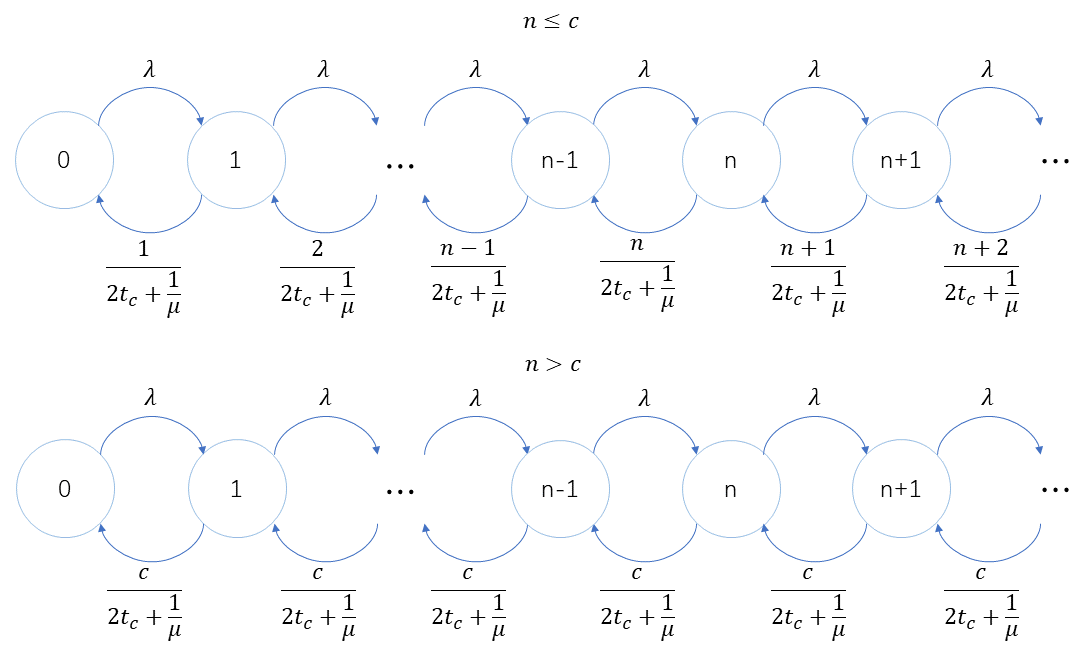
\includegraphics[width=.6\textwidth]{images/transform3.PNG}
    \caption{多通道状态转移图}
    \label{fig:transform3}
\end{figure}

对于非高峰期的多通道模型,
对应的差分方程模型如下:
\begin{equation}
    \begin{aligned}
        &\mu P_1=\lambda P_0 \\
        &(n+1)\mu P_{n+1}+\lambda P_{n-1}=(\lambda+n\mu)P_n, 1\leq n\leq c \\
        &c\mu P_{n+1}+\lambda P_{n-1}=(\lambda +c\mu )P_n, n>c
    \end{aligned}
\end{equation}

其中的$\rho=\frac{\lambda}{\mu}\geq 1$,否则队长会发散。
求解结果如下:
\begin{equation}
    \begin{aligned}
        &P_0=\Big[\sum_{k=0}^{c-1}\frac{1}{k!} \rho^k +\frac{1}{c!(1-\rho)}\cdot \rho^c \Big]^{-1} \\
        &P_n=
        \begin{cases}
            \frac{1}{n!}\rho^n P_0 \\
            \frac{1}{c!c^{n-c}}\rho^n P_0
        \end{cases}
    \end{aligned}
\end{equation}

从而求得平均对长$L_s=\frac{(c\rho)^c\rho}{c!(1-\rho)^2}P_0+\rho$

对于高峰期的多通道模型,
对应的差分方程模型如下:
\begin{equation}
    \begin{aligned}
        &\mu P_1=\lambda P_0 \\
        &(n+1)\mu P_{n+1}+\lambda P_{n-1}=(\lambda+n\mu)P_n, 1\leq n\leq c \\
        &c\mu P_{n+1}+\lambda P_{n-1}=(\lambda +c\mu )P_n, n>c
    \end{aligned}
\end{equation}

其中的$\rho=\frac{\lambda}{\mu}\geq 1$,否则队长会发散。
由于队列的容量有限,用$N=C_{queue}$,所以有限制$\sum_{k=0}^{N}P_k=1$
求解结果如下:
\begin{equation}
    \begin{aligned}
        &P_0=\Big[\sum_{k=0}^{c}\frac{1}{k!} (c\rho)^k +\frac{c^c\rho (\rho^c-\rho^N)}{c!(1-\rho)} \Big]^{-1} \\
        &P_n=
        \begin{cases}
            \frac{1}{n!}(c\rho)^n P_0 \\
            \frac{c^c}{c!}\rho^n P_0
        \end{cases}
    \end{aligned}
\end{equation}

从而求得平均对长$L_s=\frac{(c\rho)^c\rho}{c!(1-\rho)^2}P_0[1-\rho^{N-c}-(N-c)\rho^{N-c}(1-\rho)]+c\rho (1-\rho)$
多通道模型的非高峰期与高峰期理论求解完毕。

\subsubsection{模型建立与求解}
\par 实际情况中,往往有多条入校通道。相较于单通道,多通道的引入,使得
行人和自行车在条件允许时,可以选择更换通道,从而更快地通过校门。
在实际情况中,如果当前通道有人刷卡失败,行人会有一定的概率更换通道。
在模型中,规定:
\begin{itemize}
    \item 当相邻的网格没有被占用
    \item 当换到的网格正后方网格没有被占用时
\end{itemize}
行人将以$p_s=0.5$的概率换到相邻的网格。模拟过程中取通道数量为3,模型可视化
展示在图\ref{fig:3-lanes-model}中。
\begin{figure}[ht]
    \centering
    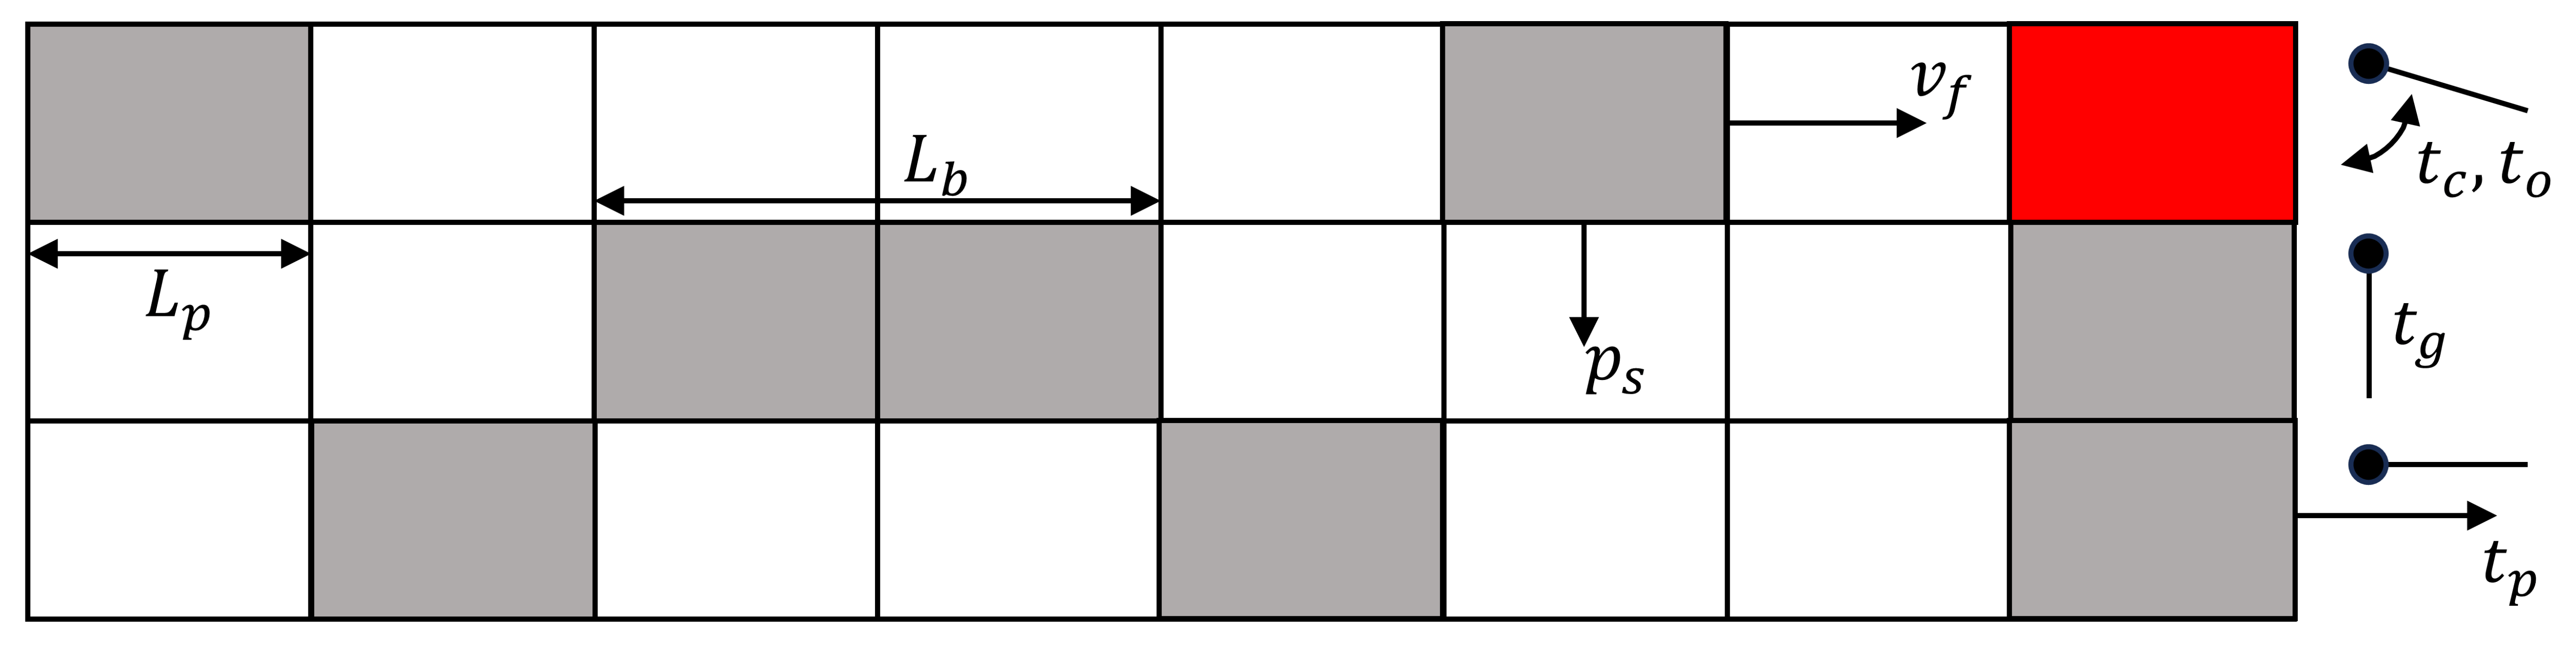
\includegraphics[width=.7\textwidth]{images/cellular_automata_3_lanes.png}
    \caption{三通道模型示意图}
    \label{fig:3-lanes-model}
\end{figure}
\par 对比多通道和单通道模型,选取1000个模拟步长,成功率0.9,分别模拟
非高峰期($\lambda_l = 0.2$)和高峰期($\lambda_h = 0.4$)的结果
展示在图\ref{fig:model-three-result}中。
\begin{figure}[ht]
    \centering
    \begin{minipage}[c]{0.45\textwidth}
        \centering
        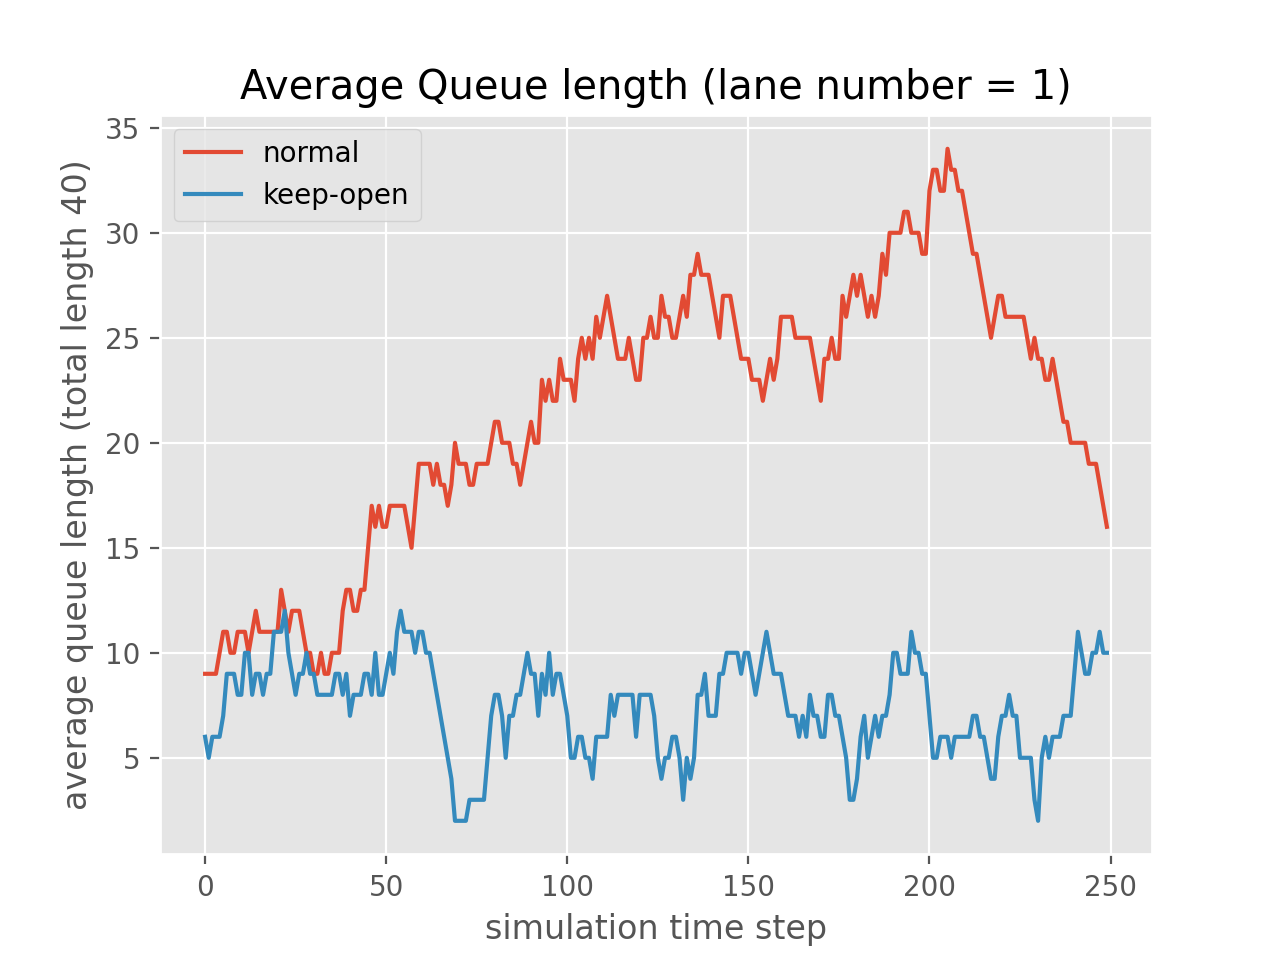
\includegraphics[width=.9\textwidth]{images/queue_length_poisson_one_lane_low.png}
        \subcaption{单通道随机模型低人流量时平均队长变化}
        \label{fig:one-lane-low-poisson}
    \end{minipage}
    \begin{minipage}[c]{0.45\textwidth}
        \centering
        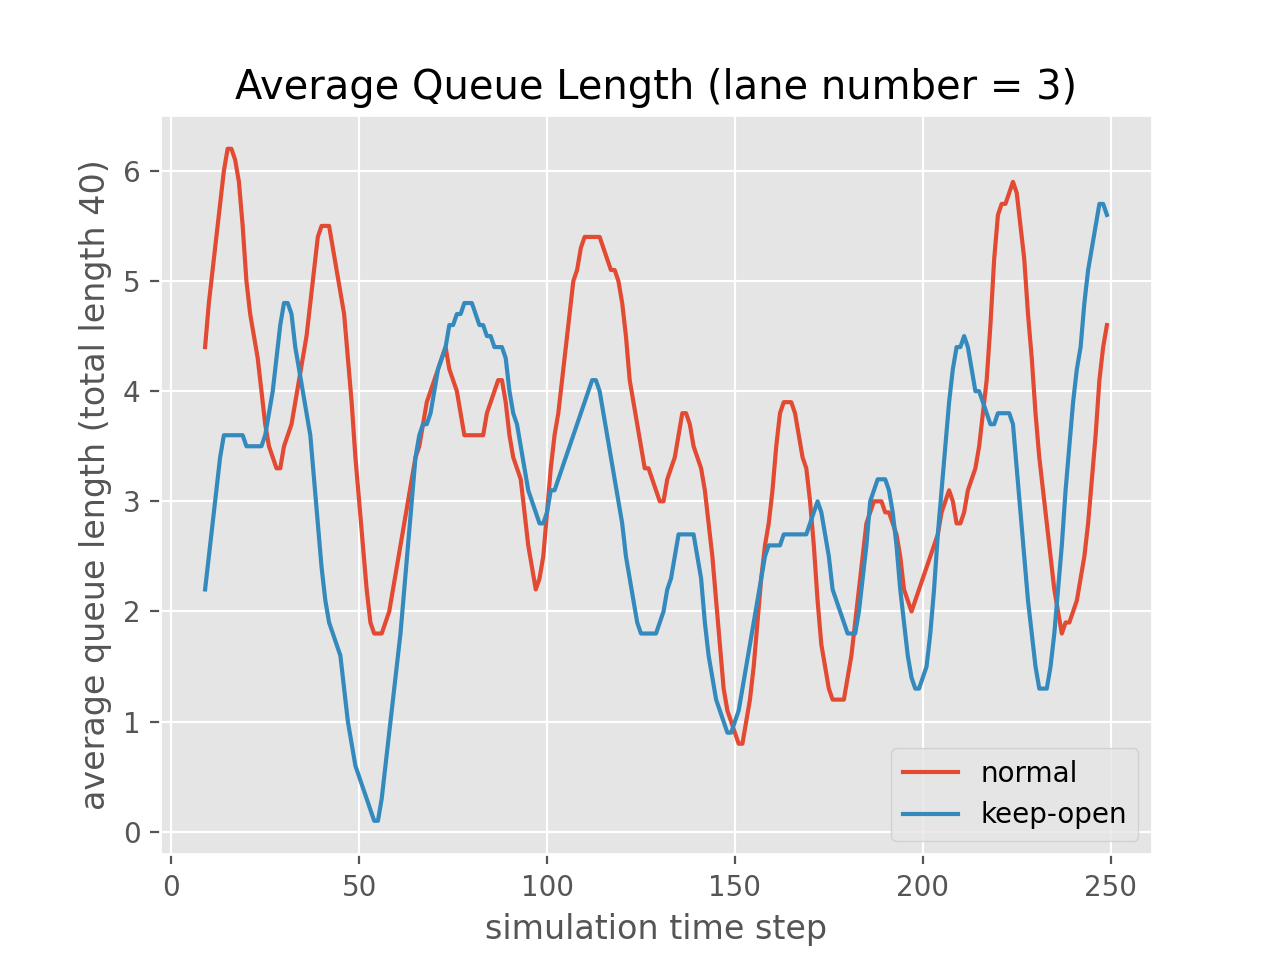
\includegraphics[width=.9\textwidth]{images/queue_length_poisson_three_lane_low_ma.png}
        \subcaption{多通道随机模型低人流量时平均队长变化(10步滑动平均)}
        \label{fig:three-lane-low-poisson}
    \end{minipage}
    \begin{minipage}[c]{0.45\textwidth}
        \centering
        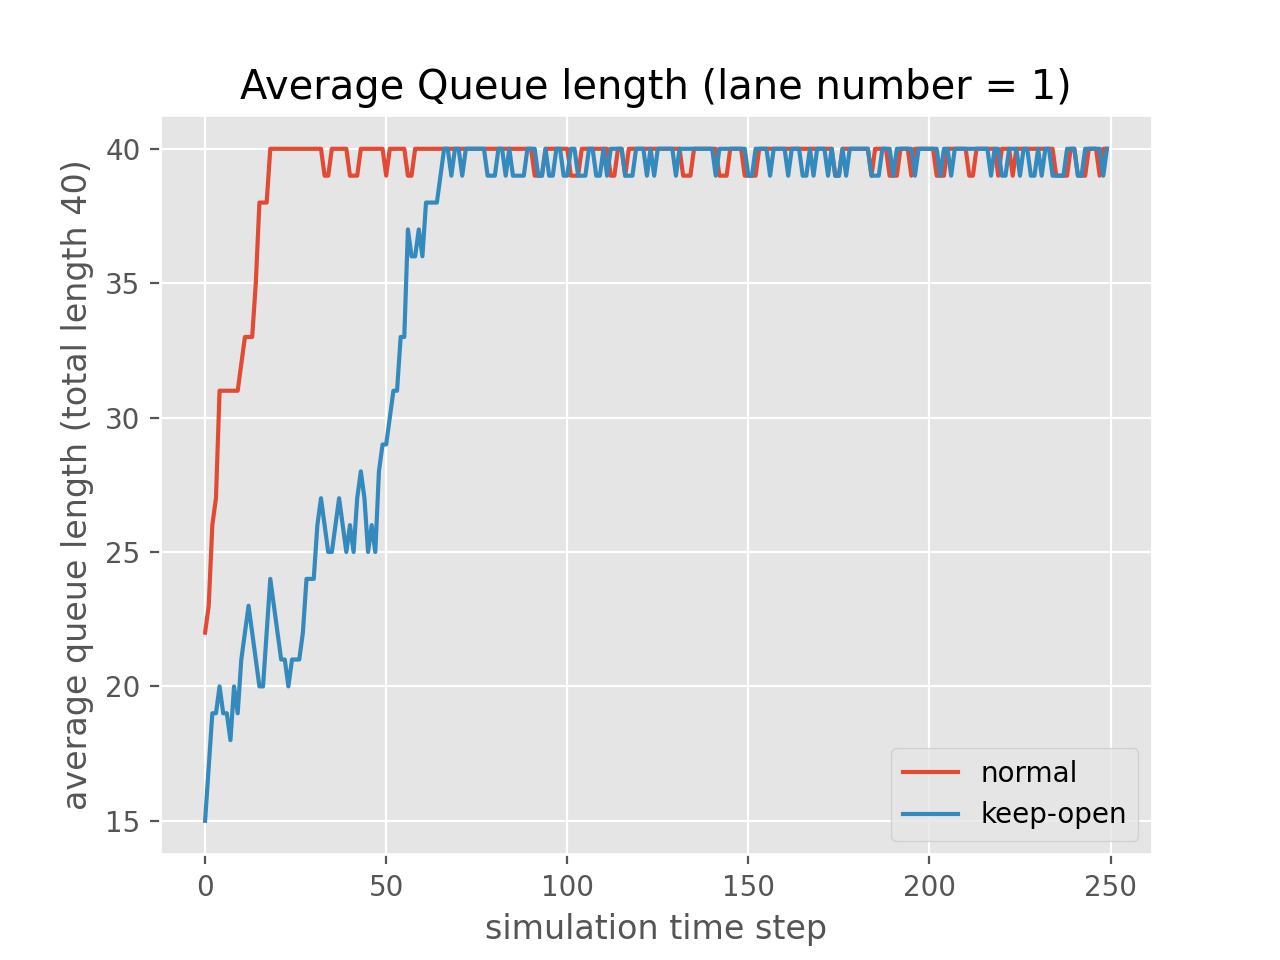
\includegraphics[width=.9\textwidth]{images/queue_length_poisson_one_lane_high.png}
        \subcaption{单通道随机模型高人流量时平均队长变化}
        \label{fig:one-lane-high-poisson}
    \end{minipage}
    \begin{minipage}[c]{0.45\textwidth}
        \centering
        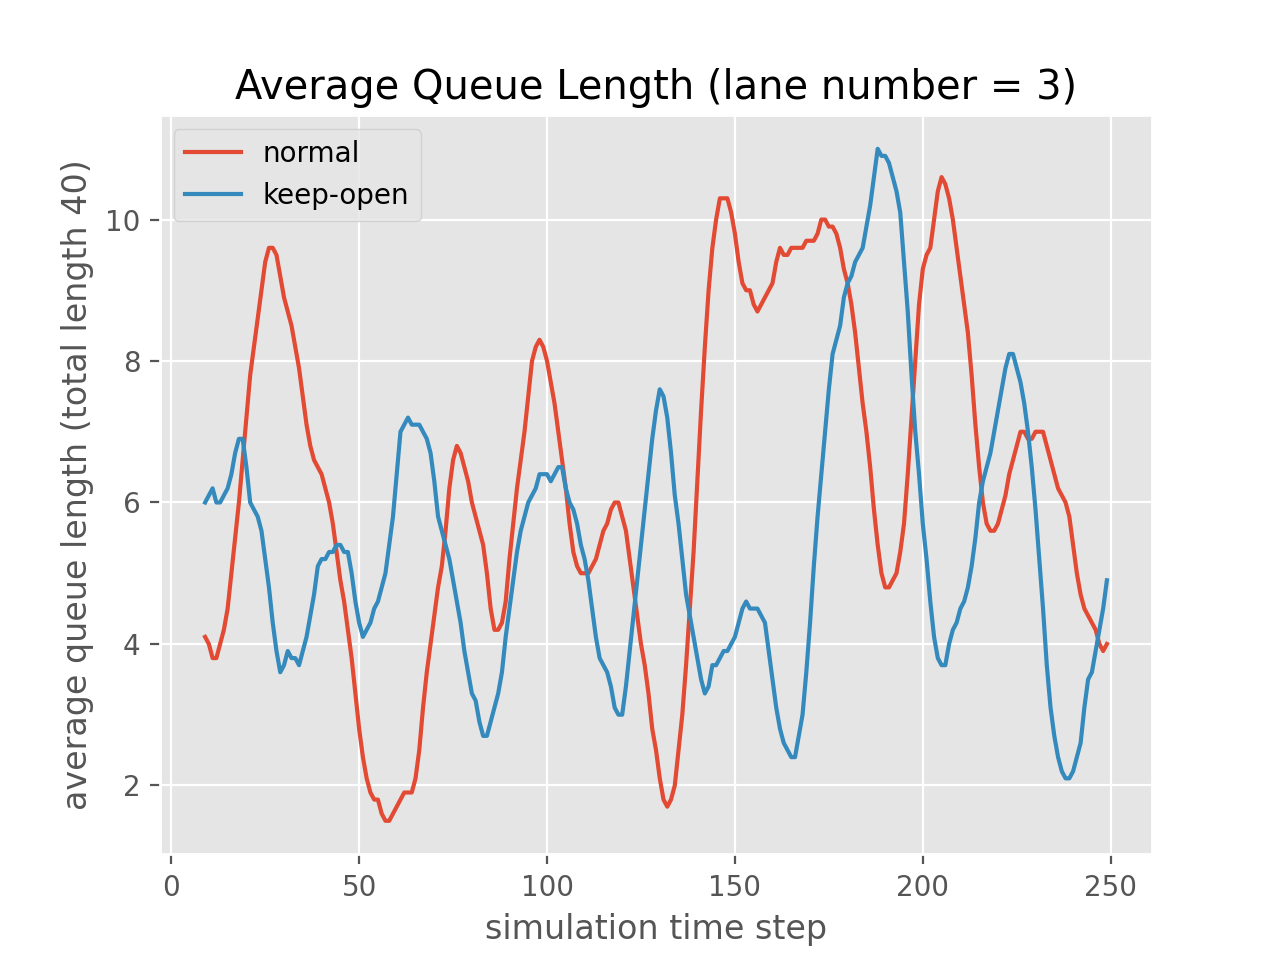
\includegraphics[width=.9\textwidth]{images/queue_length_poisson_three_lane_high_ma.png}
        \subcaption{多通道随机模型低人流量时平均队长变化(10步滑动平均)}
        \label{fig:three-lane-high-poisson}
    \end{minipage}
    \caption{多通道与单通道随机模型在高低人流量情况下平均队长对比}
    \label{fig:model-three-result}
\end{figure}
\subsection{基于数值模拟结果的通行方式建议}
\par 在非高峰期,根据模型结果,默认关门的平均队长比大约是默认开门的两倍,
通行效率显著低于后者,几乎没有可比性。在高峰期且刷卡失败率较高时,
两种通行模式的的平均队长之比趋近于1,表明两者的效率相近。而这时,
默认关门比默认开门的安全性大大提高。所以在人流较大且刷卡失败率
高的情况下,应当使用默认关门的模式。
\par 就同济大学而言,在特殊时期,例如樱花季、部分法定假期等,
人流量显著提高,且主要通行人员的身份从学生转为游客,刷卡成功率大大降低,
而且安全性也有所降低。这时使用默认关门的模式,在通行效率上没有太大的影响,
而在安全性上得到提高。而在平常时期,出入主体为学生,可以使用默认开门
的模式,提高通行效率。
\par 除此以外,此模式还可以推广到其他出入系统,如地铁站。
地铁站对于安全性的要求较高,且在客流量较大时还需要考虑管理问题,从而
需要综合考虑人流量、通行人主要成分、通行时间段等因素,
综合判断通行效率与安全性,给出对应开门方式。